\chapter{Approach and Objectives}
\label{chapter:approach-objectives}

This chapter presents an overview of the current status and future direction of
this work, with a focus on the developments and approaches to be undertaken in the
upcoming semester. In Section~\ref{section:objectives}, we summarize the overall
objective of this work, discussing the progress that has been made, as well as
the goals for the future. Section~\ref{section:timeline} provides a detailed
timeline of the tasks that have been identified and their scheduling. Finally,
in Section~\ref{section:remarks}, we offer a succinct evaluation of the
challenges encountered throughout the course of this semester.

\section{Objectives}
\label{section:objectives}

The primary objective of this project is to research and develop efficient
heuristic and meta-heuristic methods for solving optimization problems, with a
specific focus on the modeling aspect. By utilizing a modeling approach, we aim
to thoroughly understand the problem by capturing as much information as
possible, before applying meta-heuristic techniques to find solutions.
Additionally, this modeling strategy will allow for the implementation of
meta-heuristics in a problem-agnostic manner, which will be applied to a
selection of Google Hash Code problems, as outlined in the scope of this work.

During the first semester, a survey of several Google Hash Code problems was
conducted, and one problem was subsequently chosen for further analysis. The
methodology and results of this preliminary work are presented in detail in the
following chapter.

In alignment with the objective, a comprehensive review of relevant literature
and existing frameworks was conducted. Based on the principles established in
the literature review, the chosen problem was then modeled, and simple
algorithms/utilities were developed to facilitate the verification of results.
However, the analysis of the current problem is not yet complete, and further
enhancement of the results obtained with the developed model is possible from
both an implementation and conceptual perspective. This work will be continued
during the early stages of the second semester.

Additionally, we aim to select two more Google Hash Code problems for which
models will be developed. Furthermore, several state of the art meta-heuristics
will be implemented in order to experimentally evaluate the performance of the
models and to provide insight into the advantages and limitations of this
approach from both a conceptual and implementation perspective.

As the problem tackled during the first semester, as well as the additional
problems to be tackled in the future, will also be addressed through the usage
of an API~\cite{outeiro2021application}, this work has required significant
investment in the learning and utilization of said API. While the API is
generally complete, certain aspects require further refinement, and the local
search paradigm has yet to be fully integrated into it, as it was primarily
designed for constructive search. This represents a secondary objective of our
work, which will be pursued in parallel to our efforts to model the problems in
a principled manner.

\section{Timeline}
\label{section:timeline}

Given the objectives outlined in Section~\ref{section:objectives}, several
tasks were identified and are presented in the following diagram along with
their corresponding timeline:

\begin{figure}[h]
      \centering
      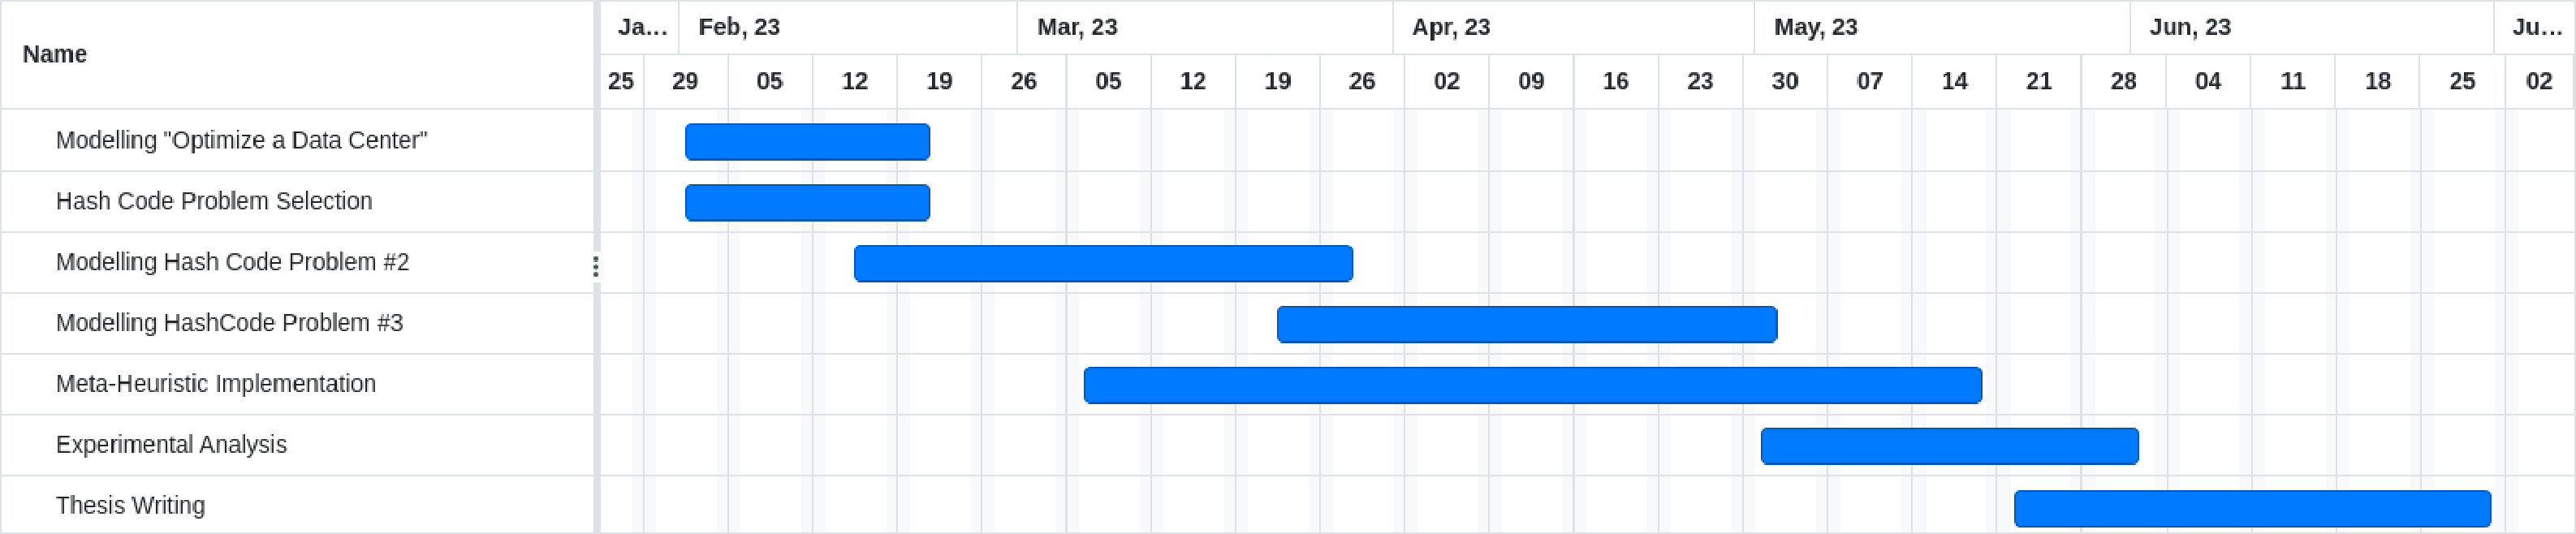
\includegraphics[width=\textwidth,keepaspectratio]{../assets/gantt/gantt.pdf}
      \caption{Project Timeline}
      \label{fig:timeline}
\end{figure}

\begin{itemize}
      \item \textbf{Modelling "Optimizing a Data Center"}: Finalize and fine-tune
            the implementation of the model for this problem.
      \item \textbf{Google Hash Code Problem Selection}: Complete the survey of the
            Google Hash Code problems and select two problems for further analysis.
      \item \textbf{Modelling Google Hash Code Problem \#2}: Develop a model for the
            first selected problem.
      \item \textbf{Modelling Google Hash Code Problem \#3}: Develop a model for the
            second selected problem.
      \item \textbf{Meta-Heuristic Implementation}: Implement state-of-the-art
            meta-heuristics to test the approach of separating model development from
            solution development and to obtain competitive solutions for the modeled
            problems.
      \item \textbf{Experimental Analysis}: Conduct a thorough experimental analysis
            of the results obtained for all problems.
      \item \textbf{Thesis Writing}: Compose the final thesis report.
\end{itemize}

\section{Concluding Remarks}
\label{section:remarks}

The previous sections (Section~\ref{section:objectives} and
Section~\ref{section:timeline}) have outlined the current approach, current
work, objectives, and tasks to be undertaken in the remaining time budget of
this project. However, it is important to note that there have been some
challenges encountered in the work already developed, and that are worth
mentioning

From a personal perspective, the shift in paradigm towards a more principled
approach to modeling presented a significant learning curve, as it is a concept
that was not previously part of my problem-solving toolkit. This may have been
due to the novel nature of the approach, which required a thorough understanding
and familiarization of the underlying concepts.

Additionally, utilizing the API~\cite{outeiro2021application} required a
significant investment in understanding its implementation and quirks that must
be considered when implementing a model. Furthermore, the API was developed in
C, while this work was conducted in C++, which required some adjustments to the
existing code. The decision to use C++ was motivated by its familiarity and ease
of use, as well as the availability of a standard library of support data
structures, which was identified as a significant improvement that would aid in
the development of models.

Lastly, in regards to the development of the API, it should be noted that the
author~\cite{outeiro2021application} has implemented certain algorithms in a
problem-independent manner. While these algorithms are functional, they still
require certain components of the model to be fully implemented. Despite this,
it is worth noting that this experience has highlighted the importance of
clearly documenting the required operations for a model to be able to utilize a
particular solver, which we intend to keep in mind as we develop our
meta-heuristic solvers